%% This is file `jasr-template.tex',
%% 
%% Copyright 2019-2022 Elsevier Ltd
%% 
%% This file is part of the 'Elsarticle Bundle'.
%% ---------------------------------------------
%% 
%% It may be distributed under the conditions of the LaTeX Project Public
%% License, either version 1.2 of this license or (at your option) any
%% later version.  The latest version of this license is in
%%    http://www.latex-project.org/lppl.txt
%% and version 1.2 or later is part of all distributions of LaTeX
%% version 1999/12/01 or later.
%% 
%% The list of all files belonging to the 'Elsarticle Bundle' is
%% given in the file `manifest.txt'.
%% 
%% Template article for Elsevier's document class `elsarticle'
%% with harvard style bibliographic references
%%
%% $Id: jasr-template.tex 226 2022-10-21 02:17:38Z rishi $
%%
%% Use the option review to obtain double line spacing
%\documentclass[times,review,preprint,authoryear]{elsarticle}

%% Use the options `twocolumn,final' to obtain the final layout
%% Use longtitle option to break abstract to multiple pages if overfull.
%% For Review pdf (With double line spacing)
%\documentclass[times,twocolumn,review]{elsarticle}
%% For abstracts longer than one page.
%\documentclass[times,twocolumn,review,longtitle]{elsarticle}
%% For Review pdf without preprint line
%\documentclass[times,twocolumn,review,nopreprintline]{elsarticle}
%% Final pdf
\documentclass[times,twocolumn,final,authoryear]{elsarticle}
%%
%\documentclass[times,twocolumn,final,longtitle]{elsarticle}
%%

%%
%% Stylefile to load JASR template
\usepackage{jasr}
\usepackage{framed,multirow}

%% The amssymb package provides various useful mathematical symbols
\usepackage{amssymb}
\usepackage{latexsym}

%% For line numbers
\usepackage[switch]{lineno}

% Following three lines are needed for this document.
% If you are not loading colors or url, then these are
% not required.
\usepackage{url}
\usepackage{xcolor}
\definecolor{newcolor}{rgb}{.8,.349,.1}

\usepackage[citebordercolor=white]{hyperref}

\journal{Advances in Space Research}

\begin{document}

\verso{Given-name Surname \textit{etal}}

\begin{frontmatter}

\title{Type the title of your paper, only capitalize first
word and proper nouns\tnoteref{tnote1}}%
\tnotetext[tnote1]{This is an example for title footnote coding.}

\author[1]{Given-name1 \snm{Surname1}\corref{cor1}}
\cortext[cor1]{Corresponding author: 
  Tel.: +0-000-000-0000;  
  fax: +0-000-000-0000;}
\author[1]{Given-name2 \snm{Surname2}\fnref{fn1}}
\fntext[fn1]{This is author footnote for second author.}
\author[2]{Given-name3 \snm{Surname3}}
%% Third author's email
\ead{author3@author.com}
\author[2]{Given-name4 \snm{Surname4}}

\address[1]{Affiliation 1, Address, City and Postal Code, Country}
\address[2]{Affiliation 2, Address, City and Postal Code, Country}

\received{1 May 2013}
\finalform{10 May 2013}
\accepted{13 May 2013}
\availableonline{15 May 2013}
\communicated{S. Sarkar}


\begin{abstract}
%%%
Please type your abstract here, and the rest of the text, figures,
tables, equations etc. in the main body. Please do not modify LaTeX\ 
commands unless you need to modify them and know how to do it.
%%%%
\end{abstract}

\begin{keyword}
%% MSC codes here, in the form: \MSC code \sep code
%% or \MSC[2008] code \sep code (2000 is the default)
%\MSC 41A05\sep 41A10\sep 65D05\sep 65D17
%% Keywords
\KWD Keyword1\sep Keyword2\sep Keyword3
\end{keyword}

\end{frontmatter}

%% For linenumbers
\linenumbers

%% main text
\section{Introduction}
\label{sec1}
Please use \verb+elsarticle.cls+ for typesetting your paper. Additionally,
make sure not to remove the package \verb+jasr.sty+ already included in the
preamble:
\begin{verbatim} 
  \usepackage{jasr}
\end{verbatim}

Make sure to have the file \verb+jasr-model5-names.bst+ to produce the references in
the correct format. 

Any instructions relevant to the \verb+elsarticle.cls+ are
applicable here as well. See the online instruction available at:
\makeatletter
\if@twocolumn
\begin{verbatim}
 https://support.stmdocs.in/wiki/
 index.php?title=Elsarticle.cls
\end{verbatim}
\else
\begin{verbatim}
 https://support.stmdocs.in/wiki/index.php?title=Elsarticle.cls
 \end{verbatim}
\fi
\makeatother

Following commands are defined for this journal which are not in
\verb+elsarticle.cls+. 
\begin{verbatim}
  \received{}
  \finalform{}
  \accepted{}
  \availableonline{}
  \communicated{}
\end{verbatim}


\subsection{Subsection}
This is only a \LaTeX\ template if you need one. 
See the detailed guidelines for manuscript preparation 
and submission at:
\begin{verbatim}
https://ees.elsevier.com/asr
\end{verbatim}

\section{Main text of your manuscript}
You like to write, don't you?

\section{How to include a figure?}
Change the file name of the figure below with your own 
figure. And remember to change the figure caption too!
\begin{verbatim}
\begin{figure}
  \centering
  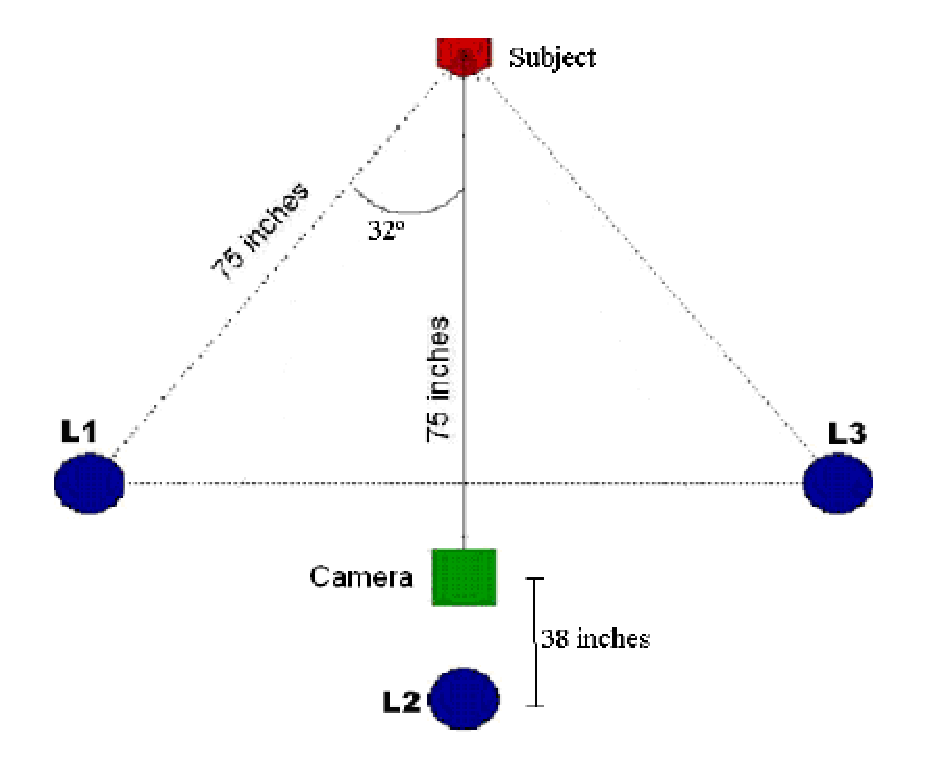
\includegraphics[scale=0.5]{fig01}
  \caption{Write the figure caption here.}
  \label{fig:pendulum}
\end{figure}
\end{verbatim}

\begin{figure}
\centering
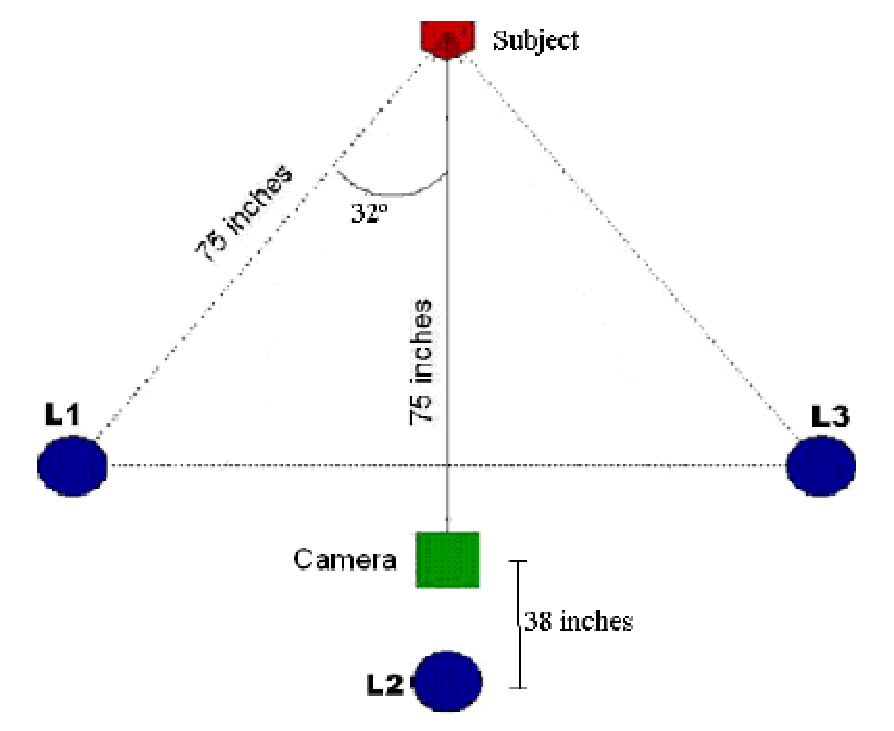
\includegraphics[scale=0.5]{fig01.pdf}
\caption{Write the figure caption here.}
\label{fig:pendulum}
\end{figure}

\subsection{And a table?}
Just replace the text/values in the template table below 
with your own. You can change the number of 
lines/rows as necessary.

\begin{table*}
\centering
\caption{Title of the table should be at the top}
\begin{tabular}{|l|l|l|l|}
\hline
Column Name1    & Column Name2 & Column Name3 & Column Name4 \\
\hline
Parameter Name1 & Value        & Value        & Value        \\
\hline
Parameter Name2 & Value        & Value        & Value        \\
\hline
Parameter Name3 & Value        & Value        & Value        \\
\hline
\end{tabular}
\end{table*}

\subsection{Equations}
Conventionally, in mathematical equations, variables and
anything that represents a value appear in italics. 
All equations should be numbered for easy referencing. 
The number should appear at the right margin.
\begin{eqnarray}
S'_{\mathrm{pg}} = \frac{S_{\mathrm{pg}} - \mathrm{min}(S_{\mathrm{pG}})}
  {\mathrm{max}(S_{\mathrm{pG}} - \mathrm{min}(S_{\mathrm{pG}}))}
\end{eqnarray}
In mathematical expressions 
in running text "/" should be used
for division (not a horizontal line).

\section{Citations}
Citations in the text can be made using\\[6pt]
\verb+\citet{NewmanGirvan2004}+\\[6pt]
for citation in running text like in 
\citet{NewmanGirvan2004} or using\\[6pt]
\verb+\citep{Vehlowetal2013,NewmanGirvan2004}+\\[6pt]
for citation within parentheses like in 
\citep{Vehlowetal2013,NewmanGirvan2004}.

Please use the actual \verb+\cite+ command in the text.
Also, please double-check the \verb+\citep+ command.

\section{Reference style}
You can include the references in the main text file in \LaTeX
format. Alternately, you can include a separate bibliography
file (refs.bib in this example) and run the following set of 
commands:
\begin{verbatim}
==================

pdflatex myfile.tex

bibtex myfile (no extension in this line!)

pdflatex myfile.tex

pdflatex myfile.tex

==================
\end{verbatim}

\section{A sample entry in the bibliography file}
%{\fontsize{7.5pt}{9.6pt}\selectfont
\begin{verbatim}
==================

@ARTICLE{NewmanGirvan2004,
  author  = {Newman, M. E. J. and Girvan, M.},
  title   = {Finding and evaluating community 
               structure in networks},
  journal = {Phys. Rev. E.},
  volume  = {69},
  number  = {21},
  year    = {2004},
  pages   = {026113}
}

==================
\end{verbatim}
%}

\section*{Acknowledgments}
Acknowledgments should be inserted at the end of the paper,
before the references, not as a footnote to the title. Use the
unnumbered Acknowledgements Head style for the Acknowledgments
heading.

%% Bibliography
%% Author year style
\bibliographystyle{jasr-model5-names}
\biboptions{authoryear}
\bibliography{refs}

\end{document}

%%

